% !TEX root = ../main.tex

% Scaling human-collected robot data has expanded the capabilities of generalist manipulation policies~\citep{o2024open,khazatsky2024droid}, but demonstration scaling alone does not close the loop between deployment and continual improvement.
Scaling human-collected robot data has expanded the capabilities of generalist manipulation policies~\citep{o2024open}, but demonstration scaling alone does not close the loop between deployment and continual improvement.
Deployment exposes states, interactions, and failure modes beyond curated demonstrations, providing new experience for an embodied data flywheel.
Real-world reinforcement learning (RL)~\citep{xu2026rlt} can improve policy performance during deployment, but may narrow the model's predictive distribution and often struggles to learn multi-task generalist policies.
Although distilling a generalist policy from multiple RL specialists~\citep{xiao2025pld} can address this issue, the generalist's supervision comes from curated successful rollouts rather than the full interaction history.
Therefore, we aim to study direct generalist improvement from the full mixture of successful, suboptimal, and failed deployment rollouts.
The challenge is to use this experience productively: imitating every recorded action risks absorbing undesirable behavior, while retaining only high-quality trajectories discards informative interactions and their outcomes.


Recent VLA and world-action models address important pieces of this problem.
On the VLA side, $\pi_{0.6}$~\citep{physicalintelligence2025pi06} uses advantage-conditioned learning to incorporate autonomous experience and interventions, while $\pi_{0.7}$~\citep{physicalintelligence2026pi07} uses quality, speed, and mistake metadata to absorb mixed-quality data and distill specialist capabilities into a generalist.
These VLA methods use steering during training to model behavior distributions across data qualities and specify a desirable mode at inference for smooth execution, but rely on VLM-based language--vision--action representations without an explicit objective for learning the physical dynamics reflected in action--video transitions.
Consequently, suboptimal and failed rollouts provide behavior targets but do not directly supervise learning of their physical consequences.
World modeling offers a more elegant solution: WAMs~\citep{pai2025mimicvideo,ye2026world,lingbot-va2026} couple predictive visual representations with action generation, while action-conditioned world models (ACWMs)~\citep{guo2025ctrlworld,gao2026dreamdojo} predict future observations conditioned on actions.
Combining the two allows ACWM to learn action consequences from data of different qualities, while WAM learns appropriate actions from expert demonstrations.
$\tau_0$-WM~\citep{zhou2026tau0wm} trains separate WAM and ACWM, routing failure and recovery data to ACWM training and use ACWM as selector for policy improvement.
FACT~\citep{peng2026fact} implements the two roles within a shared model, but retains sequential action--consequence generation. It only supports success/failure supervision split, with failure consequences influencing the policy implicitly through shared representations.
These approaches expose a remaining design challenge in learning from mixed-quality deployment experience: VLA steering lacks natural action--video dependency modeling, while consequence-aware WAMs still exploit rollout data indirectly through an ACWM interface---a simulator for action selection or a subsequent consequence-prediction stage that influences the policy through shared representations.
Can a single WAM directly learn from mixed-quality deployment rollouts, with all qualities supervising the model and learned consequences participating directly in action generation?

\begin{figure}[t]
    \centering
    % Preserve the supplied illustration with current vector result panels.
    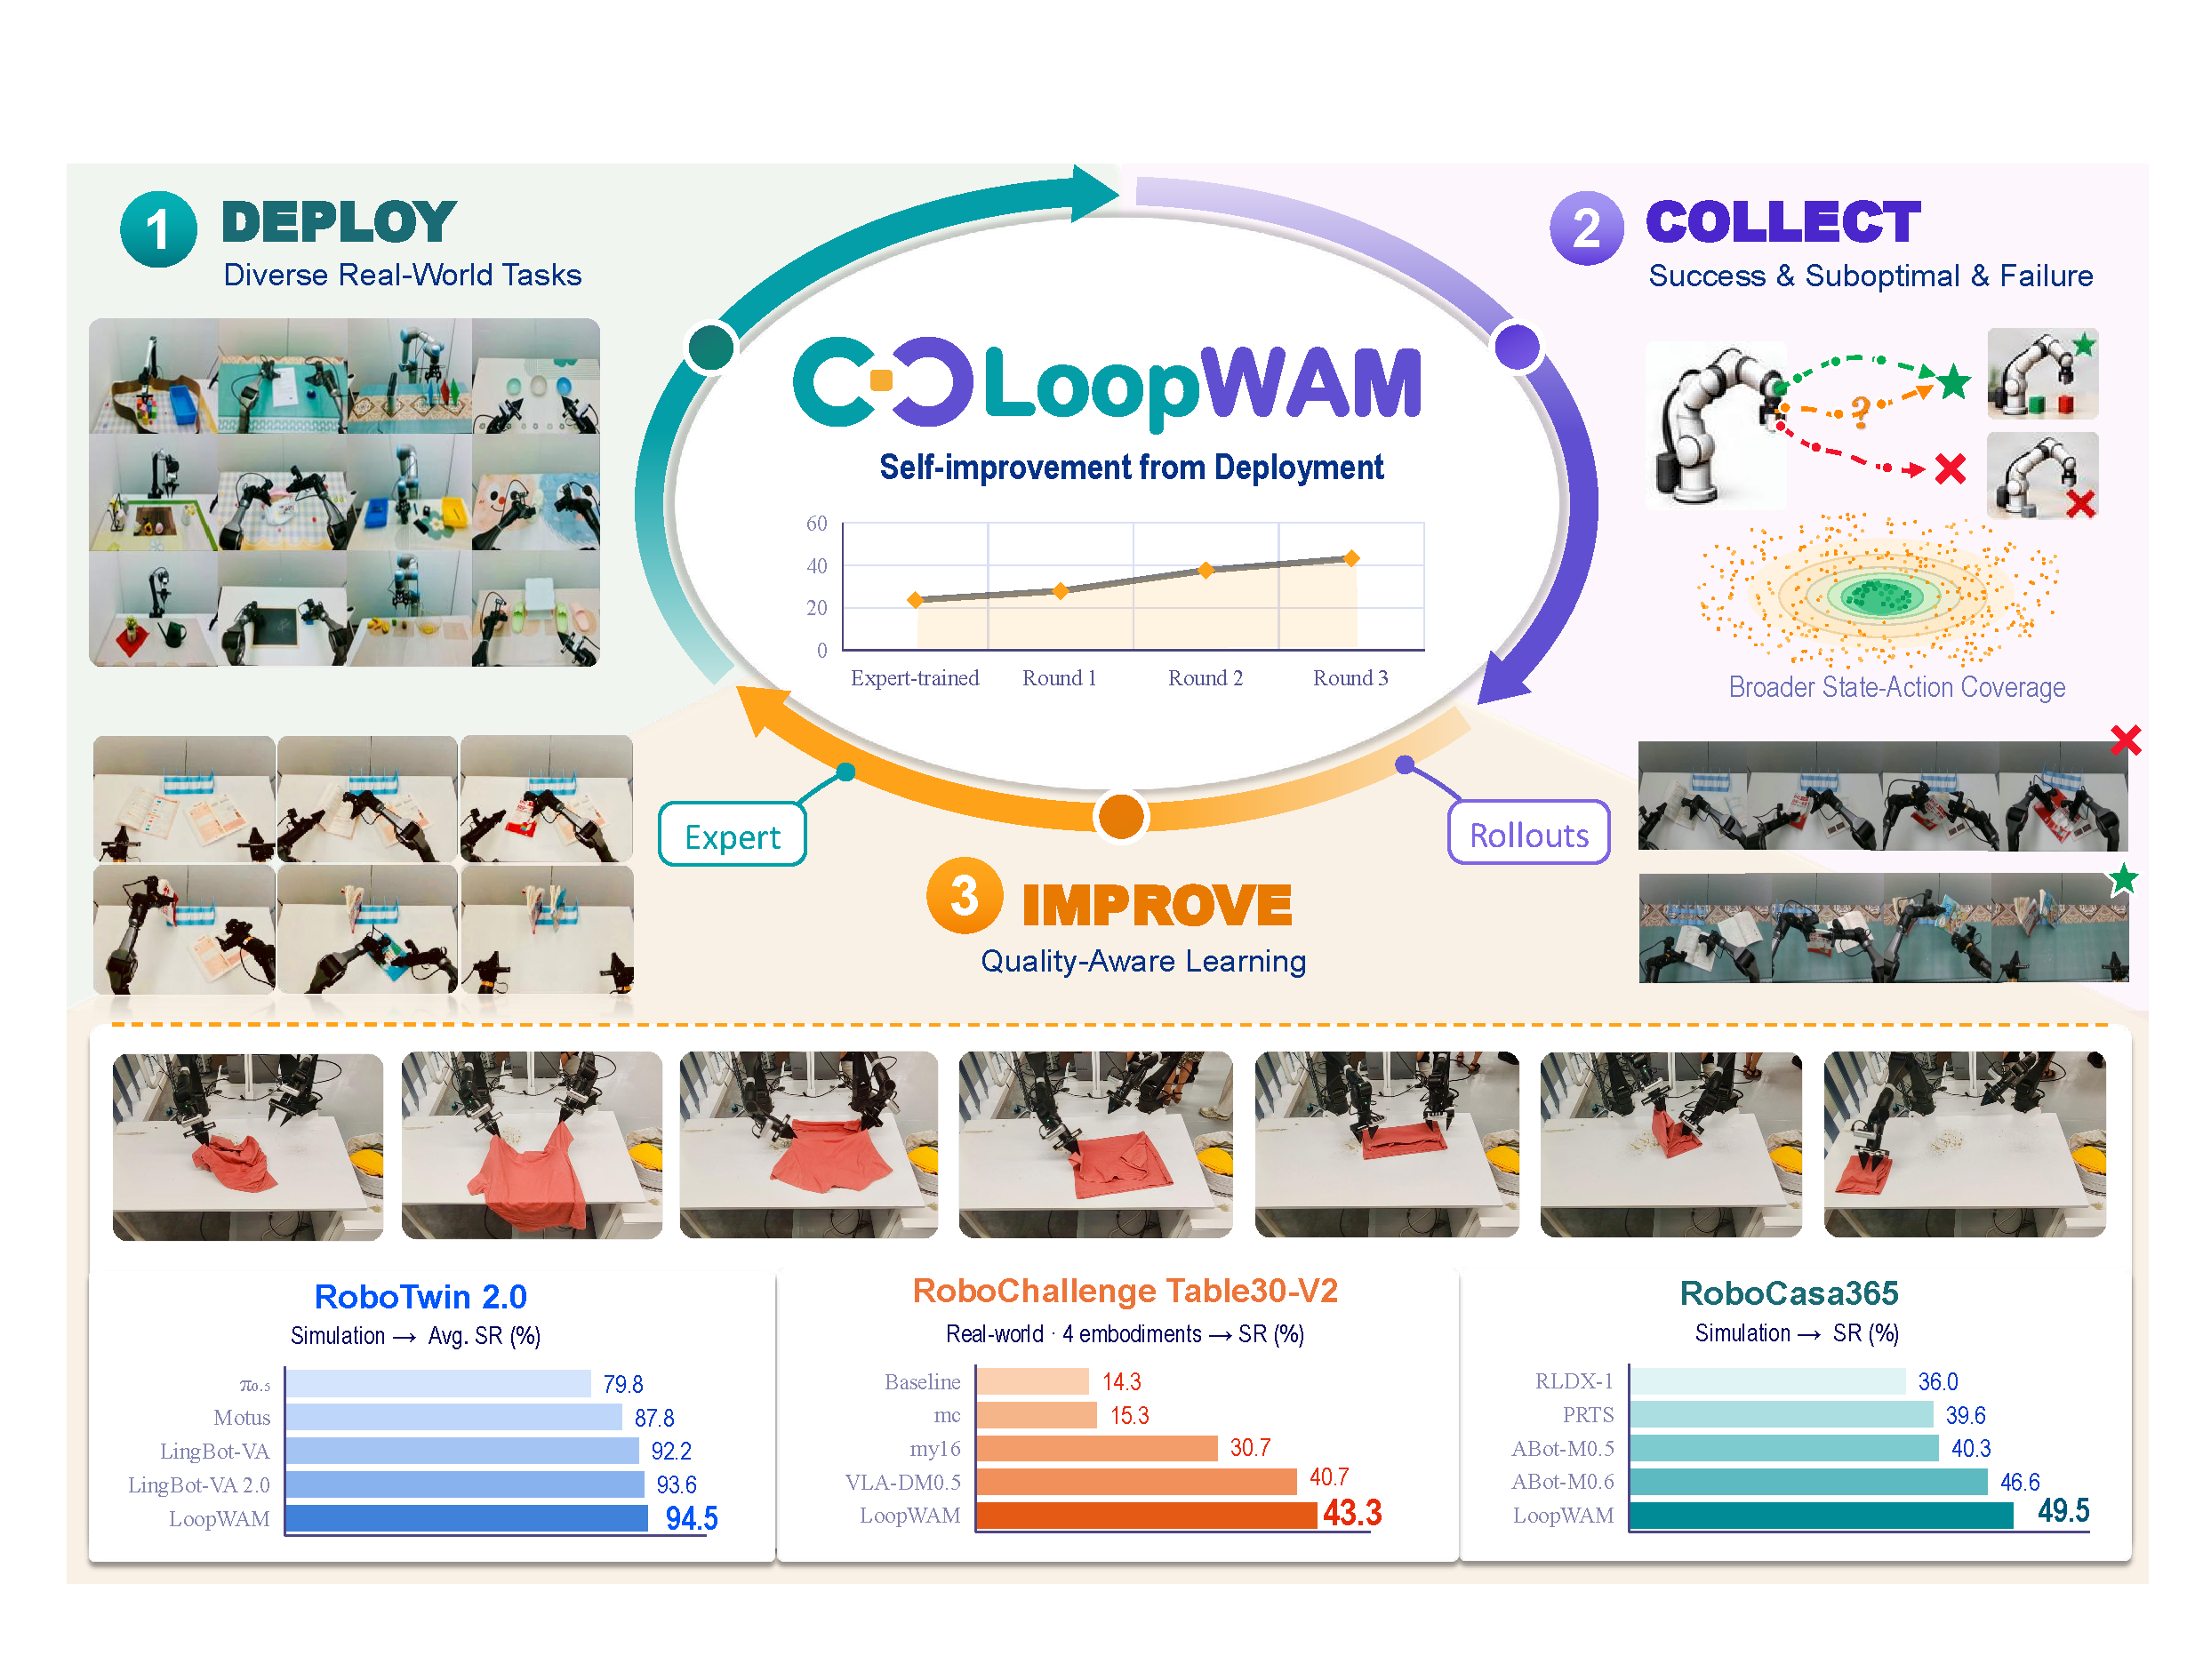
\includegraphics[width=\linewidth]{figures/teaser.pdf}
    \caption{\textbf{LoopWAM learns from deployment.}
    Mixed-quality rollouts return to training through quality steering, source-dependent noise sampling, and quality-weighted supervision.
    Center: closed-loop self-improvement on RoboChallenge Table30-V2, where three rounds of deployment and retraining increase overall success from 23.67\% to 43.33\%.
    Bottom: benchmark comparisons.}
    \label{fig:teaser}
\end{figure}


We introduce \textbf{LoopWAM}, a closed-loop World-Action Model that updates a generalist directly from mixed-quality deployment rollouts.
Our core idea is to let one WAM directly absorb rollouts across the full quality spectrum and learn from each.
To achieve this, we first use \emph{source-dependent noise sampling} to unify WAM behavior learning and ACWM consequence learning within a single model and generation stage.
Video and action noise levels are sampled independently, allowing low-noise rollout actions to guide prediction of their observed consequences.
Within this unified model, \emph{quality steering} represents behaviors of different qualities and selects the highest-quality condition at deployment.
To control how strongly each behavior is imitated, we further apply \emph{quality-weighted supervision}, reducing imitation of suboptimal actions and masking failed-action targets while retaining video supervision across all qualities.
Together, these mechanisms let every trajectory supervise the joint model according to its behavioral quality and observed transitions.
Video and action tokens interact bidirectionally throughout one parallel denoising process, allowing learned future representations to participate in action formation without a separate consequence-evaluation stage.
We close the loop by repeatedly collecting rollouts and retraining the generalist on demonstrations and accumulated experience before redeployment.
On \textbf{RoboChallenge Table30-V2}~\citep{robochallenge2026table30v2}, three rounds raise overall success from \textbf{23.67\%} to \textbf{28.00\%}, \textbf{37.67\%}, and \textbf{43.33\%}, a \textbf{19.7-percentage-point improvement}, with a final score of \textbf{56.80}, ranking first in both success and score among the compared entries (Table~\ref{tab:robochallenge_results}).
LoopWAM achieves \textbf{94.5\%} average success on \textbf{RoboTwin~2.0}~\citep{chen2025robotwin2}, exceeding the reported 87.5\% of FACT and 93.6\% of LingBot-VA~2.0, and \textbf{49.5\%} on the 50-task \textbf{RoboCasa365} evaluation~\citep{nasiriany2026robocasa365}, above ABot-M0.6's 46.6\% (Tables~\ref{tab:robotwin_results}--\ref{tab:robocasa_results}).
We further evaluate deployment-driven self-improvement after single-task post-training on challenging shirt folding, which involves deformable objects and multiple coordinated steps.
Two deployment-and-training rounds raise success from \textbf{13.20\%} to \textbf{55.56\%} (Section~\ref{sec:closed_loop_results}).
These results establish that directly learning from mixed-quality rollouts with parallel world--action denoising can deliver leading benchmark performance and repeated deployment improvement in both multi-task and single-task settings.
